\chapter{Martedì 02/03/2021}
\section{Architettura IBM-compatibile con processore Intel a 64 bit}
Iniziamo a vedere un architettura IBM compatibile con processore Intel a 64 bit. Facciamo alcune premesse.
\begin{itemize}
	\item Dire che una cosa è uscita in un certo anno non significa dire che quella cosa sia stata inventata in quel momento. Certe volte si sente dire che Steve Jobs o Bill Gates hanno inventato il computer, e ciò è una castroneria.
	\item A partire dagli anni 70 si è avuto un processo di miniaturizzazione, che ha portato ad avere calcolatori di dimensione minore, accettabili per l'uso domestico.
\end{itemize}
\paragraph{IBM} Nel 1981 l'IBM decide di entrare nel mercato dei personal computer. Inizia a commercializzare l'IBM PC 5150 e brevetta il personal computer. Il successo è stratosferico, e la concorrenza sbaragliata. 
\begin{center}
	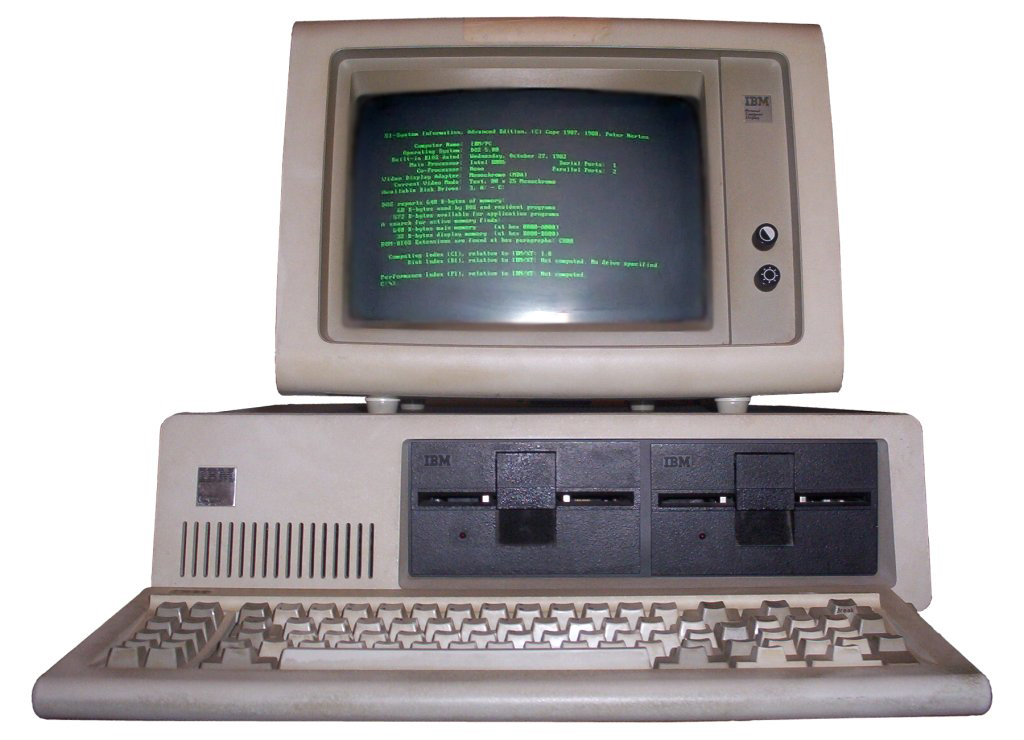
\includegraphics[scale=.25]{img/130.PNG}
\end{center}L'architettura era aperta, quindi fu possibile creare cloni legali detti \emph{IBM compatibili}. Il processore scelto dall'IBM fu l'8088 dell'Intel. 
Si tenga conto che i personal computer, inizialmente, erano molto meno potenti rispetto ai calcolatori per uso professionale. Nel tempo i PC sono stati dotati di tutte le funzionalità che all'epoca erano presenti solo sui calcolatori per uso professionale (interruzioni e protezioni sono cose che non sono state inventate con i PC).
\subsection{Sviluppi del processore INTEL}
\begin{multicols}{2}
	\small
	\begin{itemize}
		\item \textbf{8088 16bit}, con le interruzioni
		\item \textbf{80286 16bit}, con interruzioni e protezione
		\item \textbf{80386 32bit}, con interruzioni, protezione e memoria virtuale
	\end{itemize}
	\normalsize
	\columnbreak
	\begin{center}
		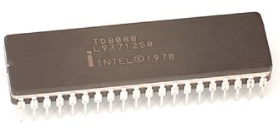
\includegraphics[scale=.75]{img/131.PNG}
	\end{center}
\end{multicols}
\noindent Dopo il terzo modello indicato non si hanno più novità rilevanti. Le novità da allora hanno riguardato soprattutto nuovi set di istruzioni e modifiche interne per velocizzare il processore. Verso la fine degli anni 90 la Intel ha introdotto \emph{Itaniun} per passare da 32 bit a 64 bit. In contemporanea la AMD ha sviluppato un'estensione dell'architettura Intel esistente, nota come \emph{AMD64}. L'Itanium non ha avuto successo e la Intel ha reso i suoi processori compatibili con l'estensione AMD.

\paragraph{Brutture} L'architettura che andremo a vedere è brutta, complicata e irregolare, vittima del suo successo. Il software sviluppato, imponente, è cresciuto negli anni principalmente per motivi di retrocompatibilità. Molte scelte del passato sopravvivono anche oggi in questi processori. 
\subsection[{Confronto col Manchester Baby}]{Confronto col Manchester Baby\footnote{Sono consapevole che questa sezione risulterà un po' antipatica. Riguardatevi modo la struttura del calcolatore). }} Facciamo un confronto con quanto visto ieri.
\begin{itemize}
	\item \textbf{CPU}: il meccanismo di esecuzione delle istruzioni è sostanzialmente simile.
	\begin{itemize}
		\item Prelievo l'istruzione,
		\item eseguo l'istruzione, e
		\item passo all'istruzione successiva.
	\end{itemize}
	La differenza sostanziale sta nella dimensione dell'istruzione: oggi questa è variabile, compresa tra 1 e 18 byte (dipende dai fattori già visti a Reti logiche).
	\item \textbf{Memoria}: vediamo le differenze principali.
	\begin{itemize}
		\item \textbf{Differenza di lana caprina}: memoria di maggiore dimensione
		\item \textbf{Differenze sostanziali}: 
		\begin{itemize}
			\item Nel Manchester Baby si può accedere soltanto a un'intera riga di 32bit (cioè operazioni di lettura e scrittura). Non si poteva intervenire su sottorighe.
			\item Le architetture erano sostanzialmente divise in due categorie: macchine scientifiche con accesso stile Manchester Baby (celle di dimensione ampia), e macchine ad uso commerciale con memorie organizzate a caratteri (byte che avevano dimensione di 5/6 bit). La macchina moderna ingloba entrambe le categorie:
			\begin{itemize}
				\item Ogni singolo byte ha un indirizzo (la dimensione del byte è stata standardizzata, 8 bit). 
				\item La memoria è accessibile non solo a singoli byte, ma anche a multipli del byte (\emph{word, doubleword e quadrupleword}, rispettivamente 16bit, 32bit e 64bit).
			\end{itemize}
		\end{itemize}
	\end{itemize}
	\item \textbf{I/O}:
	\begin{itemize}
		\item L'I/O non è collegato direttamente alla memoria, ma raggiungibile attraverso il bus.
		\item \textbf{Contrariamente al Manchester Baby è necessario del software}: quanto posto nella periferica rimane al suo interno e deve essere recuperato dal software per essere usato (per esempio quando vogliamo conoscere l'ultimo carattere premuto sulla tastiera). L'interfaccia appare al processore come una memoria, come un insieme di registri che possono essere letti e scritti. 
		\begin{center}
			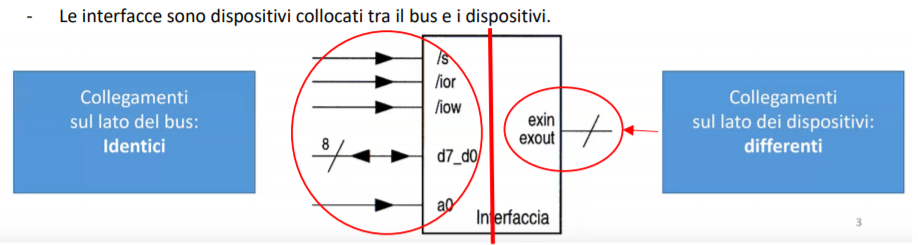
\includegraphics[scale=.75]{img/132.PNG}
		\end{center}
		La differenza importante è che operazioni di lettura e scrittura possono avere effetti collaterali sulle periferiche. 
		
		\begin{itemize}
			\item Gli indirizzi devono essere pensati come qualcosa che appartiene al bus, separato dalla memoria e dall'I/O. Gli indirizzi, tra memoria e I/O, devono essere \underline{UNIVOCI}.
			\item Un'entità attiva, per dialogare, pone sul bus l'indirizzo della cella con cui vuole parlare. Questo indirizzo è visto da tutti coloro che sono collegati al bus, \textbf{non solo da chi reagisce}.
			\item Ognuno degli oggetti collegati al bus deve sapere quali sono i propri indirizzi: in base agli indirizzi ricevuti l'oggetto capisce se deve reagire o meno. Considerando l'univocità è chiaro che in una situazione caratterizzata dalla presenza di tante periferiche solo una di queste risponderà.
		\end{itemize}
		
		\item \textbf{Attenzione}. Storicamente l'architettura prevedeva una distinzione netta tra memoria e I/O (indirizzamenti separati, ripensare alla struttura del calcolatore vista a Reti logiche). Si capiva al volo se la CPU voleva parlare con la memoria o con l'I/O. Nei pc moderni la distinzione è meno netta.
	\end{itemize}
\end{itemize}
\subsubsection{Spazio di memoria} Segue che lo spazio di memoria è una cosa diversa dalla memoria.
\begin{itemize}
	\item \textbf{Lo spazio di memoria è l'insieme di tutto ciò che è indirizzabile}, cioè degli indirizzi che il processore genera quando sta eseguendo un istruzione che ha un operando in memoria, oppure quando sta prelevando un'istruzione.
	\item Tutto ciò che è presente nello spazio di memoria può essere letto con l'istruzione MOV (ovviamente tenendo conto di meccanismi come la protezione).
\end{itemize}
\paragraph{Spazio di memoria comprende lo spazio di I/O?} 
\begin{itemize}
	\item Nell'architettura che vedremo lo spazio di I/O non è parte dello spazio di memoria: la CPU genera un indirizzo nello spazio di I/O quando esegue le istruzioni IN e OUT.
	\item Vedremo che in alcuni casi le periferiche (solitamente quelle "più vecchie") hanno i registri nello spazio di I/O, mentre altre (solitamente quelle più recenti) hanno i loro registri nello spazio di memoria (quindi vi si può accedere con una semplice MOV, basta conoscere l'indirizzo).
\end{itemize} 
\paragraph{Dunque}
\begin{itemize}
	\item La CPU genera un accesso sul bus nello spazio di memoria.
	\item Lo schema prevede che ogni sottoparte dell'oggetto collegato al bus abbia un suo indirizzo diverso: una memoria RAM occupa un intervallo di indirizzi, stessa cosa ogni signola periferica. 
	\item Una volta che l'oggetto ha capito che deve lavorare deve individuare la sottoparte chiamata in causa: prendiamo una periferica, il processore non solo vuole parlare con la periferica, ma vuole anche leggere/scrivere su uno specifico registro.
\end{itemize}
\subsubsection{Introduzione della memoria ROM, utilità della memoria ROM} Altra differenza rispetto al Manchester Baby è la presenza di una memoria ROM, oltre che di una RAM. perché ci serve?
\begin{itemize}
	\item La CPU non fa niente se non c'è del software.
	\item Dobbiamo eseguire il programma bootstrap, cioè fornire del software base. Se io non eseguo questo programma mi ritrovo con una memoria piena di spazzatura, e la CPU interpreta cose casuali come istruzioni (se possibile).
	\item Nel Manchester Baby non abbiamo un programma bootstrap, ma non è un problema visto che \textbf{possiamo inserire roba in memoria senza dover avere qualcosa già in memoria}. Nell'architettura moderna tutto è gestito dal software, incluse le periferiche di I/O: se non ho software non ho nè input nè output. Esco da questo ciclo solo introducendo una memoria di sola lettura.
\end{itemize}
\subsubsection{Differenza tra hardware e software} 
\[\boxed{\text{Il software consiste in tutto ciò che è contenuto in memoria, l'hardware è tutto il resto.}}\]
La confusione è lecita: alcune cose fatte in software potrebbero essere fatte in hardware, e viceversa
\clearpage
\subsection{Riflessioni approfondite sulla CPU} 
Abbiamo capito che il suo scopo è eseguire istruzioni in linguaggio macchina. Queste istruzioni possono fare riferimento ad operandi (ricordarsi che l'istruzione base è quella aritmetica, due operandi che producono un risultato da memorizzare da qualche parte).
\begin{verbatim}
	OPCODE source, destination
\end{verbatim}
\paragraph{Dove si trovano gli operandi?}
\begin{enumerate}
	\item In un registro,
	\item direttamente nell'istruzione (\emph{operando immediato}, costante), o
	\item nello spazio di memoria (ricordiamoci, spazio di memoria adesso è una cosa decisamente più generica).
\end{enumerate}
Per facilitare il parsing l'operando costante inizia col dollaro, mentre il registro con la percentuale. In tutti gli altri casi si ha un operando immediato. Ricordiamoci la regola fondamentale: tutto ciò che ha a che fare con una istruzione deve stare nel processore. Pensiamo al calcolatore a 32 bit visto a Reti logiche: nella fase di fetch tutto ciò che non è presente nel processore viene portato al suo interno.

\subsubsection{Spazio di memoria e regole di indirizzamento (CISC)}
Lo spazio di memoria è la cosa più complessa. L'architettura del processore è detta CISC (\emph{Complex Instruction Set Computer}): il set delle istruzioni è complesso, nel senso che una singola istruzione può fare tante cose\footnote{\textbf{Definizione della Wikipedia inglese}. A complex instruction set computer is a computer in which single instructions can execute several low-level operations (such as a load from memory, an arithmetic operation, and a memory store) or are capable of multi-step operations or addressing modes within single instructions}. Se dobbiamo generare un indirizzo nello spazio di memoria possiamo chiedere al processore di calcolarlo: le metodiche sono le stesse viste a Reti logiche (si vedano le pagine sulle regole di indirizzamento, riprese dalla dispensa di Reti logiche). Si consideri che Lettieri chiama il \emph{displacement} con un altro nome: \emph{offset}.

\subsubsection{Problema: offset dell'indirizzo a 32 bit} L'offset ha dimensione di 32bit. Si è deciso di non espanderlo a 64bit per evitare un aumento eccessivo della dimensione delle istruzioni (inutile nella maggior parte dei casi). perché la cosa è fastidiosa? Prendiamo la seguente istruzione
\begin{verbatim}
	MOV offset, %RAX
\end{verbatim}
il fatto che l'offset sia a 32bit ci permette di porre come source solo i primi 4GB di memoria. La AMD ha introdotto due modi per aggirare il problema:
\begin{itemize}
	\item l'istruzione MOVABS, l'unica istruzione che ha l'offset a 64bit.
	\begin{verbatim}
		MOVABS offset, %RAX <----- N.B. UNICO REGISTRO UTILIZZABILE
		MOVABS $costante, %RAX
		MOVABS %RAX, offset
	\end{verbatim}
	\item L'indirizzamento con registro base e offset a 32bit con segno.
	\begin{verbatim}
		offset(%RIP)
	\end{verbatim}
	che sostanzialmente equivale a dire 
	\[\text{Indirizzo}=\left|\text{base} \pm \text{offset}\right|_{\text{modulo}_{2^{64}}}\]
	ricordarsi che RIP è un registro a 64bit e che l'offset viene esteso con segno (cioè replicando il bit più significative per il numero necessario di volte). In un certo senso equivale a stabilire il punto di riferimento: da questo punto posto in RIP possiamo leggere 2GB indietro e 2GB avanti (ricordarsi del segno). Si osservi che questo tipo indirizzamento \textbf{già esisteva}, ma è stato reso esplicito per gli operandi. Era già presente nelle istruzioni di salto, introdotte così a Reti logiche:
	\begin{verbatim}
		JMP %EIP +- displacement
	\end{verbatim}
\end{itemize}
\subsubsection{Utilità degli indirizzamenti nelle strutture dati} L'idea centrale è che uno piazza le cose in memoria e accede liberamente, nel modo più semplice possibile. La cosa interessante è che attraverso certi tipi di indirizzamenti posso creare delle strutture dati e calcolare velocemente gli indirizzi delle componenti.
\begin{itemize}
	\item \textbf{Array}: l'array è un insieme di elementi consecutivi, tutti dello stesso tipo. Il dimensionamento di ogni singolo elemento è lo stesso, quindi mi basta indicare il numero di bit di ciascun elemento attraverso la scala e incrementare il registro indice ogni volta.
	\[\text{Indirizzo}=\left|\text{base} \pm \text{indice} \times \text{scala}\right|_{\text{modulo}_{2^{64}}}\]
	\item \textbf{Struttura}: ho una serie di elementi consecutivi, di dimensione diversa tra loro. Ho indirizzi diversi, ma uno scostamento costante rispetto all'indirizzo base. Questo scostamento è posto nella definizione della struttura.
	\item \textbf{Puntatore}: il puntatore equivale all'indirizzamento di tipo indiretto con registro base. bit di ciascun elemento attraverso la scala e incrementare il registro indice ogni volta.
	\[\text{Indirizzo}=\left|\text{base}\right|_{\text{modulo}_{2^{64}}}\]
\end{itemize}
\clearpage 
\subsubsection{Registri} Rispetto a Reti logiche abbiamo più registri, tutti di dimensione maggiore. Sono tutti interni al processore e sono la unità di memorizzazione più veloce che ci sia. Un registro può essere letto e scritto in un ciclo di clock, cosa assolutamente impossibile con una RAM (la lettura/scrittura può richiedere centinaia di clock). 
\begin{center}
	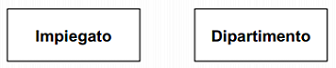
\includegraphics{img/5.PNG}
\end{center}
\begin{itemize}
	\item I registri già esistenti nell'architettura a 32bit sono stati mantenuti.
	\item Il registro dei flag è stato esteso a 64bit, ma non contiene nuovi flag. Anche l'instruction pointer è stato esteso a 64 bit.
	\item I registri rimanenti sono stati estesi e contengono la loro vecchia versione a 32bit: i nomi per richiamarle \underline{sono esattamente gli stessi}!
	\item La AMD ha uniformato gli accessi, nel senso che nei rimanenti registri a 64bit troviamo SEMPRE la versione a 16bit e 8bit (cosa che non era valida per alcuni registri, ripensare a Reti logiche). 
	\item Resta una irregolarità: solo i registri A, B, C, D sono accessibili anche nella parte più significativa dei primi 16bit (AH, BH, CH, DH), gli altri sono accessibili solo nella parte meno significativa.
\end{itemize}
A differenza del manchester baby abbiamo (cose già viste a Reti):
\begin{itemize}
	\item istruzioni che alterano in modo implicito il registro stackpointer (per esempio la chiamata di funzione, tutto ciò che è legato alla pila);
	\item istruzioni che alterano il registro dei flag settandoli (per esempio STD e CLD);
	\item istruzioni che verificano se sono presenti specifiche configurazioni di flag e decidono, conseguentemente, se fare salto o meno (JMP condizionate, il Manchester Baby prevedeva un JMP condizionata molto primitiva\footnote{Verificare se il numero posto nel registro accumulatore è positivo o negativo, dunque fare un eventuale salto DI UNA SOLA ISTRUZIONE.}).
\end{itemize}